\subsubsection{Def. P, NP, NP-hard \& NPC}

Lad os nu kigge på de kompleksitetsklasser vi har arbejdet med her i kurset.
\begin{center}
 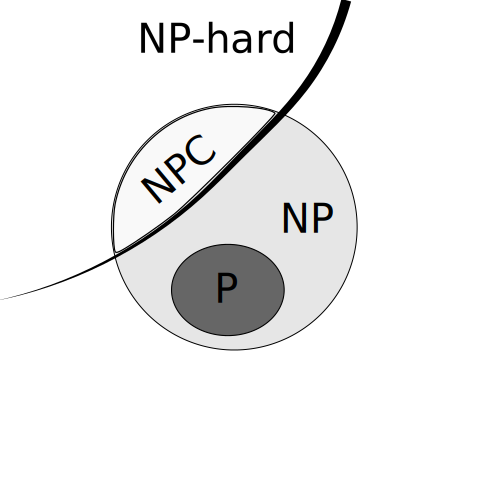
\includegraphics[bb=0 0 400 400,scale=0.3]{./PNPNPC.png}
 % PNPNPC.png: 1667x1667 pixel, 300dpi, 14.11x14.11 cm, bb=0 0 400 400
\end{center}


\paragraph{P}
~\\
~\\
Kompleksitetsklassen $P$ er formelt defineret således:
\begin{align*}
 P = \left\lbrace L \subseteq \left\lbrace 0,1 \right\rbrace^* | \exists \text{ TM } M_L \text{ der afgører L i polynomiel tid } \right\rbrace
\end{align*}
Altså klassen af beslutningsproblemer der kan blive bestemt af en deterministisk Turing Maskine hvor antallet af ``steps'' maskinen udfører for et givent $x$ maksimalt er $\rho(x)$ for et givent polynomiel $\rho$.\\
 
Intuivit ser vi kompleksitetsklassen $P$ som en klasse for problemer for hvilket vi kender en effektiv løsning. Altså ethvert problem med worst-case kørselstid på formen $O(n^k)$ for et givent $k$.

At worst-case kørseltid på et problem er polynomiel betyder dog ikke reelt at det er et nemt problem (modsat hvad Cobham's Thesis påstår). I hele den analyse ignorerer vi fuldkommen konstanter, samt forventet kørselstid som I mange tilfælde kan få ``sværere'' problemer til at køre bedre end ``nemme'' problemer i $P$.


\paragraph{NP}
~\\
~\\
Kompleksitetsklassen $NP$ er lidt mere kluntet formelt defineret, så vi starter lige med intuitionen først.

Intuitivt kan $NP$ ses som klassen af beslutningsproblemer for hvilket ``yes'' instanserne kan verificeres i polynomiel tid på en deterministisk Turing Maskine. Altså er det komplekse problemer med eksponentiel løbetid, men hvor løsningen til et sådant problem nemt kan verificeres til at være korrekt.\\
~\\
Kompleksitetsklassen $NP$ er formelt defineret således:
\begin{align*}
  NP = \left\lbrace L \subseteq \left\lbrace 0,1 \right\rbrace^* |
    \exists \rho \in Z[x], L' \in P, \forall x \in \left\lbrace 0,1
    \right\rbrace^* : ( x \in L \Leftrightarrow \exists y \in
    \left\lbrace 0,1 \right\rbrace^* : |y| \leq \rho(|x|) \wedge
    \left\langle x,y \right\rangle \in L') \right\rbrace
\end{align*}
Definitionen skal forståes således: Vi har et sprog $L' \in P$, samt et polynomiel $\rho$. Vi tænker så nu på et sæt af binære strenge af længde maksimalt $\rho(|x|)$, hvor disse representerer mulige løsninger til probleminstansen $x$. Med denne fortolkning bliver $\left\langle x,y \right\rangle \in L'$ så måden hvorpå vi tester om en given løsning $y$ virkelig er en korrekt løsning. 

Denne form for søgningsproblem kaldes ofte for et simpelt søgningsproblem, da den kan verificeres i polynomiel tid, men ikke løses deri (antaget $P \neq NP$).\\

For at løse et givent NP problem kunne vi så løbe igennem alle mulige løsninger for $y$, som sammenlagt ville være $2^{\rho(|x|)+1}-1$, og for hver af dem tjekke $\left\langle x,y \right\rangle \in L'$. Det ønsker vi dog ikke, da det ville tage eksponentiel tid. I stedet forsøger man ofte at finde snedige måder at lave speed-ups og/eller lave approximationsalgoritmer af forskellige art.

Og i visse tilfælde er man også heldig at finde en algoritme i $P$ for et $NP$ problem, hvorved man har vist at problemet i virkeligheden ligger i $P$ som jo er et subset af $NP$.

\paragraph{NP-hard}
~\\
~\\
Et sprog defineres som NP-hard såfremt der gælder:

\begin{align*}
 \lbrace L \subseteq \lbrace 0,1 \rbrace^* | \forall L' \in NP: L' \leq L \rbrace
\end{align*}

Altså gælder der, at ethvert sprog $L'$ i NP kan reduceres til $L$. Intuitionen er her, at algoritmen til at løse NP-hard problemet er så stærk (eller generel) at den kan bruges til at løse ethvert andet problem i NP. Man siger desuden, at et NP-hard problem således er mindre sandsynlig end noget andet sprog i NP, til at være i P.\\

Navnet kan dog være lidt forvirrende, da et NP-hard problem faktisk ikke behøver være i NP og hvis de er, så kaldes de faktisk ikke engang bare NP-hard længere.

\paragraph{NPC}
~\\
~\\
NP-Complete (NPC) er den særlige klasse af problemer der både er NP-hard og befinder sig i NP. Formelt defineret således: 

\begin{align*}
 NPC = \left\lbrace L \in \left\lbrace 0,1 \right\rbrace^* | L \in NP \wedge (\forall L' \in NP: L' \leq L) \right\rbrace
\end{align*}

NPC problemer er særligt interessante, da vi kan bruge dem til at bevise et givent problem er NP-Complete, således vi ikke spilder tid på forsøg med at finde en algoritme i $P$ for problemet (antaget $P\neq NP$). Dette gør vi vha. noget vi kalder reduktioner, som bygger på polynomial time computable maps.

